%
%
%
%
%
%
%
%
%
%
%
%
%
%
%
%
\begin{document}
\maketitle
\begin{abstract}
\end{abstract}

\section{Introduction} 

% (fold)
\label{sec:introduction}

Suppose that you wanted to make the following argument: 
\begin{hypo}
	\label{h1} A particular property of a brain causes a particular mental property. 
\end{hypo}

The ``brain property'' could be nearly anything: the genetic expression profile of a subset of neurons in a particular developmental stage, or microtubules becoming entangled, or columnar organization, or the bumps in our skulls, etc. Similarly, the ``mental property'' could be almost anything: intelligence, capacity for love, knowing the square-root of pi, etc. How might you go about \emph{proving} Hypothesis \ref{h1} (H\ref{h1})?

Here's how we would do it. First, we would change H1 to be \emph{testable}, and change our desiderata from \emph{proving} its accuracy to \emph{collecting evidence} to support its claim. More specifically, we would make the following argument:
\begin{hypo}
	\label{h2} A change in particular property of a brain can predict a corresponding change in a particular mental property\footnote{Note the relationship between this and \emph{statistical-supervenience}\cite{VogelsteinPriebe10}}. 
\end{hypo}

Now, to collect evidence in support of H\ref{h2}, we need the following:
\begin{enumerate}
	\item A way to describe any brain, $b$. Our description should live in the space of all possible descriptions of brains (or, at least those under consideration), $\mB$. 
	\item A way to describe a mental property, $m$, which lives in the space of mental properties, $\mM$. For instance, if the mental property under investigation is IQ, then $\mM$ may be all possible scores on a particular IQ test. 
	\item A mapping from brain space to mental space, which enables us to relate $m$ and $b$. Call this mapping, $g$, so $g: \mB \mapsto \mM$. 
\end{enumerate}

If we choose to take a statistical perspective, then both brains and minds are random variables. More specifically, let $B$ be a random variable corresponding to a brain, so that any particular brain, $b$, is a sample from the space of brains, $\mB$. The probability of $B$ taking any value $b \in \mB$ is given by the \emph{marginal} distribution $F_B[b = B]$%, where $\int_{b\in\mB} F_B[b=B]db=1$, and $P_B[b=B]\geq 0 \, \forall b \in \mB$
. Similarly, let $M$ be a random variable corresponding to the mental property under investigation, so $m$ is a sample from the space of mental properties, $\mM$. The probability of $M$ taking any value $m \in \mM$ is given by the \emph{prior} distribution $F_M[m = M]$. The mapping, $g$, tells us the relationship between any $m$ and any $b$. Or, more formally, the mapping tells us about the \emph{posterior} distribution of minds given brains, $F_{M|B}[m=M | b=B]$. 

If we knew the \emph{joint} distribution of minds and brains, $F_{BM}[b=B,m=M]$, and the marginal distribution of brains, $F_B$, then finding the mapping from brains to minds would be trivial: we would simply use Bayes rule to obtain the posterior, $F_{M|B} = F_{BM}/F_B$. However, in practice these distributions are typically unknown. Therefore, we must \emph{estimate} $g$ from a corpus \emph{data}. Assume we have collected $n$ brain/mental pairs. Then, define the corpus of data as the collection of all such pairs: $\mD_n=\{(b_1,m_1), \ldots, (b_n,m_n)\}$. The estimated mapping, $g_n$, then takes a new brain and the old \emph{training data}, and makes predictions about the mental property $m$. Formally, $g_n: \mB \times (\mB, \mM)^n \mapsto \mM$, so $g_n(b; \mD_n)=\hm$.

This work contributes a perspective on a possible space of brains, $\mB$, and several principled ways of choosing $g_n$. In so doing, we also describe a set of desiderata for both $\mB$ and $g_n$ to satisfy. We make no claim that our definitions or desiderata are novel or unique. Rather, the novel contribution (if any), is the overarching statistical perspective that unifies previously (potentially) disparate ideas into a single coherent framework.

% section introduction (end)
\section{A possible description of brains with certain desirable properties} 

% (fold)
\label{sec:B}

Many possible spaces for the descriptions of brains exist. For instance, phrenologists thought that the ``sulci and gyri'' of the \emph{skull} were sufficient to explain various mental properties, including intelligence. The space of brains they considered then, were all possible skull shapes. Clearly, such a space is not sufficient to compare the evidence support phrenological theory with an alternate theory, such as it is the sulci and gyri of the \emph{brain} that determine those mental properties. So, can we enumerate a set of desiderata which we would use to select our brain-space? Here is a possible set:
\begin{enumerate}
	\item $\mB$ should be sufficiently large to be able account for whatever properties of the brain are casually related to the properties of cognition under investigation. 
	\item $\mB$ should be sufficiently large to be able span multiple \emph{levels of explanation}. That is, we might want to be able to compare a hypothesis about the role of genetic expression profiles with another hypothesis about default mode networks. 
	\item $\mB$ should be only as large as necessary, and no larger. In particular, if we do not believe that total brain volume can \emph{cause} a particular mental property, that it need not be included. 
	\item The properties of any particular brain, $b\in \mB$, should be either measurable or estimatable, such that experimental observation may be used to obtain them.	% \item Parameter estimates should be consistent \cite{} %, that is, $\hbth_n \conv \bth$ as $n \conv \infty$.
	\item $\mB$ should admit algorithms that (are guaranteed to be able to) capture the relationship of interest. 
	\item $\mB$ should also admit \emph{causal} studies, which entail modifying a particular $b \in \mB$, to modify the corresponding mental property, $m \in \mM$. 
\end{enumerate}

Note that the above desiderata are neither complete nor unique; rather, they provide (hopefully) a reasonable set of criteria for evaluating any proposed $\mB$. 
% \section{Paradigms of research} (fold)
% \subsection{Current Paradigm}
% 
% The dominant paradigm of quantitative neuroscience in the 20$^{th}$ century has been the ``signal processing'' framework \cite{}.  Essentially, the brain is a box, that filters some stimulus, to produce some response (see Figure 1). This framework leads to the following goal:
% 
% \begin{goal}
% 	Learn the filter that the brain performs on stimuli to result in the actualized responses.
% \end{goal}
% 
% \begin{figure}[h!]
% \centering 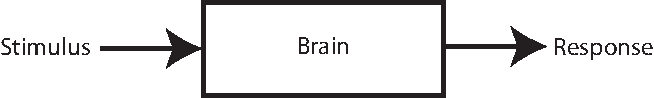
\includegraphics{stim_brain_resp}
% \caption{The signal-processing paradigm of quantitative neuroscience.  The brain is a box that essentially \emph{filters} the stimulus, outputting some response, which is often take to be multivariate time series (such as populations of spike trains or fMRI activity).} \label{fig:SBR}
% \end{figure}
% 
% 
% This paradigm has been appropriate, given the kind of data available to people investigating the brain.  More specifically, the kind of data that has been most available has been time-series of signals related to neural activity \cite{}.  Given that electrical engineers were largely the individuals obtaining and analyzing the data, it was natural to take a signal-processing approach.  Often, the dynamic time-series data were used to estimate static parameters.  In the previous decades, these communities have been more and more sophisticated models and algorithms to estimate these parameters \cite{}.  Recently, issues such as parameter identifiability, consistency, bias, and model selection have been gaining traction as important desiderata for our models \cite{}.  
% 
% \subsection{Alternate Paradigm}
% 
% Here, we define a different goal, which suggests a complementary research paradigm to the current dogma: %which we believe has not been satisfied by any previously proposed research paradigm.  Further, we elaborate on a novel paradigm that we believe is sufficient to satisfy this goal.
% 
% \begin{goal}
% 	Construct a family of brain-models, $\mB$, that is sufficient to provide \emph{causal} explanations relating properties of minds with properties of brains.
% \end{goal}
% 
% Note how the above goal is distinct in certain respects from the ``filtering'' goal.  First, neither stimulus nor response is explicitly incorporated into this goal.  While stimuli and response may be used as tools to obtain the parameters of $\mB$, that is their only merit in this paradigm.  Second, minds are explicitly incorporated into this goal.  While spike trains or fMRI signal may indicate mental processes, they are likely not what is meant by ``mind''; rather, they may be used as tools to infer mental states.  Third, the inclusion of a class of models $\mB$  suggests a statistical \emph{static} framework, rather than a dynamics perspective.  In addition to the above stated goal, we would like the family of models $\mB$ to satisfy a number of desiderata:
% 
% \begin{enumerate}
% 	\item $\mB$ %$=\{\mathbb{P}_{\bth}; \bth \in \bTh\}$ 
% 	should be sufficiently general to account for whatever properties of the brain are casually related to the properties of cognition under investigation.
% 	\item The properties of any particular brain, $b\in \mB$, should be either measurable or estimatable, such that experimental observation may be used to obtain them.
% 	% \item Parameter estimates should be consistent \cite{} %, that is, $\hbth_n \conv \bth$ as $n \conv \infty$.
% 	\item $\mB$ should admit algorithms that (are guaranteed to be able to) capture the relationship of interest.
% 	\item $\mB$ should also admit \emph{causal} studies, which entail modifying a particular $b \in \mB$, to modify the corresponding mental property, $m \in \mM$.
% \end{enumerate}
% 
% \section{NeuroCognitive Graph Theory}
% 
% \subsection{Brain-graphs}
% 
% Here, (end)
With this in mind, we propose the notion of a \emph{brain-graph}. Specifically, we say that the brain may be well characterized as a labeled, attributed multigraph (which is a generalized notion of a or network). Formally, we define a brain-graph, $b\in \mB$ as a 4-tuple, $\mB=(\mV,\mE,\mX_V, \mX_E)$, defined by the following:
\begin{itemize}
	\item The set of vertices (nodes), $V=\{V_i\}_{i\in[n_v]}$. If we assume, for instance, that neurons are the fundamental (atomic) unit of computation, then each vertex could correspond to a neuron. Regardless of what vertices represent, formally, we let $V_i \in \mV_i = \{0,1\}$ for $i \in [n_v]=\{1,2,\ldots,n_v\}$, $n_v \leq \infty$, and $\mV = \mV_i^{n_v}$.	%$=\{V_i\}$, where $V_i \in \mV \subseteq \mathbb{Z}$ . 	
	\item The set of edges, $E=\{E_{ij}\}_{i,j \in [n_v]}$. Again, if we assume that neurons are the fundamental unit of computation, then each edge could correspond to a synapse. To simplify matters we may only consider the presence or absence of a synapse, in which case $E_{ij} \in \{0,1\}$. Or, we may consider the effective strength of a synapse, in which case $E_{ij} \in \mathbb{Z}$, where $\mathbb{Z}$ is the set of integers, $\{0,1,2,\ldots\}$. Further, we could allow for the possibility of multiple ``kinds'' of synapses between any pair of neurons, such as chemical and electrical. In such a case, we have $E_{ijk} \in \mE_{ijk} \subseteq [n_v]^2 \times [n_k]$, where $n_k\leq \infty$ is the maximum number of categorically different edges. In any case, we can define the space of edges as $\mE=\mE_{ijk}^{n_v^2 \times n_k}$. 	%, where $E_{ij} \in \mE_{ij} \subseteq \mathbb{Z}$ for $(i,j) \in [n_v] \times [n_v]$, so $\mE = \mE_{ij}^{n_v^2}$.  If edges are undirected, then $E_{ij}=E_{ji}$.  If edges are binary, then $\mE=\{0,1\}$.  If we have multi-edges corresponding to categorically different edges (such as electrical and chemical synapses), each edge may also be indexed by $k \in \mathbb{Z}$. If multi-edges correspond to integer weighted edges, then $\mE$ is the set of allowable integers (which may be countably infinite).
	\item If vertices have features (or labels/attributes), then let $X_i$ correspond to the feature vector for vertex $i$ %, and define $X=\{X_i\}_{i \in [n_v]}$. 
(features may correspond to \emph{anything} about the vertex). Again, assuming vertices represent neurons, features may indicate neurotransmitter released, morphological properties, receptive fields, etc. Formally, $X_i \in \mX_1 \subseteq \Real^{d_V}$ for $i \in [n_v]$, and $d_V$ is the dimensionality of the feature vectors, so $\mX_V = \mX_1^{n_v}$. It may be the case that certain features are measurable/observable, and others are hidden. If so, let $X_i = X^o_i \cup X^h_o$, and $X^o_i \cap X^h_i = \emptyset$. 
	\item If edges also have features, then let $X_{ij}$ correspond to the feature vector for edge $(i,j)$.  If edges are synapses, then edge features might include things like probability of release, post-synaptic potential shape, etc. Let $X_{ij} \in \mX_2 \subseteq \Real^{d_E}$ for $(i,j) \in [n_v] \times [n_v]$, and $d_E$ is the dimensionality of the edge features, so $\mX_E=\mX_2^{n_v^2}$. In the scenario where categorically different edges exist, let an additional index $k$ indicates edge features for each category $k$, so $\mX_E=\mX_2^{n_v^2 \times n_k}$.
\end{itemize}

Given such a brain-space $\mB$, a natural question is: does this notion of brain-graphs satisfy the above desiderata? Let's see:

\begin{enumerate}
	\item The space of all possible brain-graphs does appear to be quite large, potentially incorporating many small and large details of brains.
	\item Because each vertex $V_i$ could correspond to a neuron, a column, a neuroanatomical region, etc., indeed, brain-graphs can span multiple levels of explanation.  Even for a given brain, it is possible to let some $V_i$'s represent neurons, and other $V_i$'s represent neuroanatomical regions, even if this is a redundant characterization of the brain, in that the neurons are \emph{within} the neuroanatomical region.
	\item While the brain-graph space is large, it is not ``all-encompassing.''  For instance, the space of all possible functions is not within brain-graph space. Thus, the brain-graph space seems to exclude at least some possibilities.
	\item For a space to admit algorithms guaranteed to capture the relationship of interest, one must prove limiting results.  For instance, Stone proved in 1977 \cite{Stone77} that the $k_n$ nearest neighbor algorithm is guaranteed to converge to the Bayes optimal solution.  In 2010, Vogelstein et al. \cite{VogelsteinPriebe10} proved a similar result holds for brain-graphs.
	\item Brain-graphs clearly admit causal studies, as one could modify the number of nodes, or the value of edges or features, and (potentially) observe a corresponding change in a mental property.  
\end{enumerate}

Thus, it seems that brain-graphs indeed satisfy the above criteria.  This is not to say that brain-graphs are the only space one could define to satisfy these criteria, merely that brain-graphs are sufficient. So, given such a space of brains, the next question is: ``how can one choose a mapping between brains and minds?''


%Assume, for the moment, that we take the fundamental computational unit of the brain to be a point neuron. Then, each vertex is a neuron, and each edge is a synapse. Categorically different edges may correspond to chemical and electrical synapses. Vertex attributes could include neurotransmitter released, proteins expressed, morphological properties, receptive fields, etc. Edge attributes could include probability of release, post-synaptic potential shape, etc. This level of description, however, is not necessary. For instance, $\mV$ might instead correspond to neuroanatomical regions, which admit very different notions for edges and attributes. This multi-scale aspect of $\mB$ is an important advantage over other frameworks. 

% section a_possible_description_of_brains_with_certain_desirable_properties (end)
\section{Possible approaches to choosing mappings with desirable properties} 

% (fold)
\label{sec:possible_approaches_to_choosing_mappings_with_desirable_properties}

Given $\mB$, what can we do with it? As stated above, our goal is to relate these models to properties of cognition. More specifically, let $\mM$ characterize the space of the mental (cognitive) property, and $g \in \mG$ be some mapping to learn. Then:
\begin{itemize}
	\item If $\mM=\{0,1\}$, then $g$ may be a two-way classifier: $g: \mB \conv \{0,1\}$. 
	\item If $\mM=\{0,1,\ldots, n_m\}$, then $g$ may be an $n_m-$way classifier: $g: \mB \conv \{0,1,\ldots,n_m\}$. 
	\item If $\mM=\Real^a$, then $g$ is a (multivariate-) regressor: $g: \mB \conv \Real^a$. 
\end{itemize}

In general, solving the above problems---which means finding $g$---will depend on the joint distribution of brains and minds, $F=F_{BM}$. In practice, however, $F$ is typically unknown, and therefore $g$ must be estimated from the data. Assume we have a corpus of training data, $\mD_n=\{(B_1,M_1), \ldots, (B_n, M_n)\}$, where $n$ is the number of training samples. Our goal then is to compute $g_n: \mB \times (\mB, \mM)^n \conv \mM$, which takes as input an observed brain-graph $b$ and $n$ training paris $\{(b_1,m_1), \ldots, (b_n,m_n)\}$ and produces a prediction $\hm=g_n(b; \mD_n)$. The particular $g_n$ should be the one that minimizes some loss function, $L_F(g_n)$, over the space of all possible $g_n$'s, $\mG$. For instance, when $|\mM|=2$, $\mG$ is all possible two-way classifiers, and a potentially reasonable loss function is $L_F(g_n)=\mathbb{E}[P_F[g_n(B;\mD_n) \neq M | \mD_n]]$.

Importantly, in addition to finding a $g_n$ that minimizes some loss-function, $g_n$ should admit a way to \emph{morph} any brain's mental property $m$, by modifying $b$. This will be discussed at greater length in the sequel. 

% \subsection{Finding a good $g_n$} % (fold)
\label{sub:finding_a_good_g_n_}

Thus, given a mental property, a decision about how to represent it, $\mM$, and a loss function, $L$, our task is to find a good algorithm, $g_n$. Two complementary strategies are possible: model-free and model-based. Model-free algorithms have the advantage that no model need be specified. Thus, in theory, model-free algorithms have the advantage of having little or no bias. Unfortunately, this freedom comes with the cost of relatively high variance. On the other hand, model-based algorithms can significantly reduce variance, but (almost) necessarily increase bias. Importantly, many standard algorithms, including linear, quadratic, and support vector based classifiers/regressors \emph{implicitly} define a model, and are therefore not strictly ``model-free''.

\subsection{Model-free algorithms} 

% (fold)
\label{sub:model_free_algorithms}

Model-free algorithms often operate on interpoint distance space, as opposed to the explicit data space \cite{MaaBartoszynski96}. More formally, given any two brain-graphs, $b_1$ and $b_2$, first define an interpoint (pseudo-) distance metric: $\rho: \mB \times \mB \mapsto [0,\infty)$. This reduces the problem from operating in $\mB$ to operating in $\Real$. Because the data collected is often corrupted by noise, it is typical to also introduce a smoothing function: $s: \mB \mapsto \mB$. For the brain-graph scenario, this may correspond to inferring unobserved edges. Thus, the smoothing-derived (pseudo-) distance metric, $\rho'$ is defined as: $\rho' = \rho(s(b_1),s(b_2))$. 

Perhaps the prototypical model-free algorithm is the $k_n$ nearest neighbor (kNN) algorithm. Vogelstein et al. (2010) showed that a kNN classifier is a universally consistent classifier (meaning, achieves the Bayes optimal performance), for any $F_{BM}$, under a Frobenius norm distance metric. In other words, they let defined $\rho(\cdot)=\norm{\cdot}_F$, and $s$ was simply the identity (that is, no smoothing). Simulations showed that for only a few hundred simulated sample data points, this kNN achieved misclassification error rate below 10\%. In practice, it is often the case that other model-free algorithms outperform (in accuracy) any particular kNN, including class cover catch digraphs, decision trees, and various ensemble approaches such as random forests \cite{}. Unfortunately, scant theoretical works is available to provide proofs of universal consistency for these alternate model-free algorithms.

%While this is a desirable property, our belief is that other $g_n$'s may outperform the kNN classifier on finite data sets.  More specifically, while kNN induces no bias whatever into $g_n$, the variance is large.  Thus, by incorporating neuroscientific knowledge about these brain-graphs into $g_n$, it may be possible to only marginally increase the bias, but drastically reduce the variance, yielding improved performance.  
% subsection model_free_algorithms (end)
\subsection{Model-based algorithm} 

% (fold)
\label{sub:model_based_algorithm}

The other possible strategy is to propose a class of models, $\mP=\{P_{\bth} : \bth \in \bTh \subseteq \Real^d\}$, that describe the data (note that the choice of how to determine the dimensionality $d$ of the model specifies whether the model is parametric, semiparametric, or nonparametric). Ideally, the class of models is sufficiently large to include models very close to the ``truth'', and be able to find a Minimally Sufficient Model (MSM; by analogy with minimally sufficient statistics) within the class, that sufficiently explains the data, with the ``smallest'' $\bTh$ (a potentially useful measure of size is the set cardinality). %goes to infinity as $n$ goes to infinity.   The advantage of using a semiparametric model is the amount of bias introduced by the model is a function of the amount of data available, that is, given infinite data, they can be bias free. The goal then is to find a Minimally Sufficient Model (MSM; by analogy with minimally sufficient statistics), which is the brain-graph with the least parameters that explains the mental property under investigation sufficiently.  %$g_n$ then operates directly on $\hbth$, the data dependent estimate of the model parameters, $\bth$. 
Classification/regression with $g_n$ is then performed on the estimate of $\bth$, which lives in some $\bTh$ space smaller than $\mB$, thereby reducing the variance, without increasing bias too much (hopefully). The model-based approach also (potentially) offers the advantage of \emph{interpretability}, if the parameters, $\bth$, correspond to interpretable features of the brain. 

Let $b_i$ correspond to brain-graph $i$. The model-based approach then typically assumes that each $b_i$ is sampled identically and independently from some parametric distribution, $b_i \overset{iid}{\sim} P(b_i | \bth) \, \forall i \in [n]$. Because $\bth$ is typically unknown, an estimate, $\hbth$, must be found. Given such an estimate, $g_n$ operates directly on the estimated parameters, as opposed to the brain-graphs \footnote{Is it interesting to note that neither paradigm actually operates directly on the data? The model-free approach operates}

The maximum likelihood approach then specifies to find The task is then to find an estimate $\hbth$, such that
\begin{align}
	\hbth = \argmax_{\bth} \prod_{i\in [n]} P(b_i | \bth) 
\end{align}

If a prior over the parameters is specified

\paragraph{Generative Model}

Consider the following generative model for attributed multigraphs:
\begin{itemize}
	\item Let $c$ be a \emph{class identity}, where $c \in \mC=\{0,1,\ldots, C\}$. The distribution of class identity, which is a random variable, is given by $f_c=MN(\bpi)$, where $MN$ indicates a multinomial, and $\bpi=(\pi_1, \ldots, \pi_)$ 
	\item Let $\bth_c$ be the \emph{parameters} for class $c$, where $\bth_c \in \bTh \subseteq \Real^{d}$, for some $d=d_{V}+d_{E} \in \mathbb{Z}$, where the dimensionality of the parameters is implicitly a function of the data, $\mD_n$. 
	\item Let $b$ be a \emph{brain-graph}, where $b(\bth_c) \in \mB=(\mV, \mE, \mX_V, \mX_E)$, where for clarity, we restrict edges to be integer weights (i.e., only include a single category of edge attributes, but this may straightforwardly generalized)	%,  Note that, for simplicity, we have dropped $\mX_E$.
\end{itemize}

To sample graphs from this generative model, assuming that $C$ and $V$ are given (the number of classes and vertices per graph, respectively), one can use the following procedure (generalizing to the unknown $V$ case is straightforward and therefore omitted):
\begin{itemize}
	\item sample $c \sim f_c$ 
	\item sample $\bth_c \sim f_{\bth}(\cdot | c)$ 
	\item for $i \in [n_v]$, sample $X_i \sim f_{X_V}(\cdot | \bth_c^V)$ 
	\item for $(i,j) \in [n_v] \times [n_v]$ 
	\begin{itemize}
		\item sample $X_{ij} \sim f_{X_E}(\cdot | \bth_c^E)$ 
		\item sample $E_{ij} \sim f_E(\cdot | X_i, X_j, X_{ij})$ 
	\end{itemize}
\end{itemize}

% \begin{algorithm} (fold)
% \caption{Pseudocode for sampling static class conditional attributed multigraphs.} \label{alg:1}
% \begin{algorithmic}[1]
% \STATE sample $c \sim P(c)$
% \STATE sample $\bth_c \sim f_{\bth}(\cdot | c)$
% \FOR{$i \in [n_v]$}
% \STATE sample $X_i \sim f_{X_V}(\cdot | \bth_c)$
% \ENDFOR
% 
% \FOR{$(i,j) \in [n_v] \times [n_v]$}
% \STATE sample $X_{ij} \sim f_{X_E}(\cdot | \bth_c)$
% \ENDFOR
% 
% \FOR{$(i,j) \in [n_v] \times [n_v]$}
% \STATE sample $E_{ij} \sim f_E(\cdot | X_i, X_j, X_{ij})$
% \ENDFOR
% \end{algorithmic} 
% \end{algorithm} (end)
Note that we have partitioned $\bth_c$ into $\bth_c^V$ and $\bth_c^E$. The probability of obtaining any graph, when using this procedure, is therefore given by:
\begin{align}
	\label{eq:G} P(G | C,V) = \left(\prod_{i,j \in [n_v]} f_E(E_{ij} | X_i, X_j, X_{ij}) f_{X_E}(X_{ij} | \bth_c^E) \right) \left(\prod_{i \in [n_v]} f_{X_V}(X_i | \bth_c^V) \right) f_{\bth}(\bth_c | c) f_c(c) 
\end{align}

Evaluating Eq. \ref{eq:G} requires defining $f=\{f_c, f_{\bth}, f_{X_v}, f_{X_E}, f_E\}$ (note that $f_{\bth}$ implicitly depends on defining $\bTh \subseteq \Real^d$, which, in turn, requires a rule for deciding $d$ based on the data). The most natural choice for $f_c$ is a multinomial, that is, $f_c = MN(\vpi)$, where $\bpi = \{\pi_1, \ldots, \pi_C\}$, $\pi_c>0$, and $\sum_c \pi_c = 1$. Our task is then to choose the rest of $f$ that yields: (i) models that display the properties of the data, and (ii) are statistically tractable, meaning that $\bth$ may be estimated consistently from the data \footnote{The above generative framework generalizes and unifies previously proposed stochastic graph models, including Random Dot Product Graphs, stochastic block models, etc.}. To proceed, we first write the posterior of interest. Importantly, it is often the case that some attributes and edges are hidden. Define $\bE=\{E_{ij}\}_{i,j \in [n_v]}$, and let $\bE = \bE^h \cup \bE^o$, where $\bE^h$ corresponds to hidden edges, and $\bE^o$ corresponds to observed edges. Similarly, let $X = X_V \cup X_E$, and then $X= X^h \cup X^o$. Finally, define $\bth=\{\bth_c\}_{c \in [C]}$. Thus, we are interested in estimating/maximizing:
\begin{align}
	\label{eq:post} P(\bth, X^h, \bE^h | C, V, X^o, \bE^o) \propto ... 
\end{align}

Several strategies for maximizing Eq. \ref{eq:post} are possible. First, one could use a Gibbs sampling strategy, iteratively sampling $\bth$, $X^h$, and $\bE^h$. Second, one could use an expectation maximization algorithm, recursively finding the expected values for $X^h$ and $\bE^h$, and then use them to estimate $\bth$. The precise definition of $f$ might necessitate approximating both these strategies. Alternately, greedy or variational approaches might be more efficient.

% subsection model_based_algorithm (end)
\subsection{Classification problem} 

% (fold)
\label{sub:classification_problem}

Imagine we are in the classification setting. What does it mean that $P(B | M=0) \neq P(B | M=1)$? It must mean that, for some subset of edges, the distribution is different for brain-graphs in the two different classes. More formally, let $S=\{(i,j) | (i,j) \in S\}$. If class conditional posteriors are different, then it must be the case that $P(\{E_{ij}\}_{(i,j) \in S} | C=0) \neq P(\{E_{ij}\}_{(i,j) \in S} | C=1)$. Given the above class of models, we may write:
\begin{align}
	P(\{E_{ij}\}_{(i,j) \in S} | c) &= f(\cdot | X, \bth_c) \nonumber \\
	&= f_E(\cdot | X) f_X(\cdot | \bth_c) f_{\bth}(\cdot | c) \nonumber \\
	&= f_E(\cdot | X) f_{X^h}(\cdot | X^o, \bth_c) f_{\bth}(\cdot | c) 
\end{align}

Thus, given a specification for $f$, the task is to find $S$, estimate the parameters $\bth$, compute the likelihood under the two models, and compare. Finding $S$, however, is, in general, non-trivial.

% subsection classification_problem (end)
% RDPG (fold)
% \begin{description}
% 	\item[Random Dot Product Graphs]  Let $\bTh = \Real^d$, and $f_{X_V}$ be the identity function, $f_{X_E}$ is a constant, and $f_E=f(\langle X_i, X_j \rangle)$, where $\langle \cdot , \cdot \rangle$  indicates a dot product
% \end{description}
% To make this a fully \emph{generative mode}, we must propose a distribution from which the $X_i$'s are sampled.  Assuming $X \in \Real^d$, then we could let each $X_i$ be sampled from a multivariate normal, that is, let $X_i \sim \mN(\mu_i,\Sig_i)$.  To be more general, we could concatenate all $X_i$'s, $\vbX=[X_1, \ldots, X_V]$, and proposed that $\vbX \sim \mN(\vmu, \vSig)$.  Imposing constraints on $\Sigma$ (such as block-diagonal) reduces this more general model to the previous one.  If we are in the classification setting, with $z$ classes, the goal then is to estimate $\vmu_z$ and $\vSig_z$, for all $z=1,\ldots, Z$.  The class of $b$ is then the $m_z$ with the highest posterior.  Thus, a natural advantage of a fully generative model is that it admits a principled loss function.  
% 
% \paragraph{Random Dot Product Graphs}
% 
%  One particularly compelling model is the Random Dot Product Graph (RDPG), where the value of an edge between two vertices is a function of the dot product between the vertex attributes.  For binary adjacency matrices, for example, we have $P[E_{ij} | X_i, X_j]=f(X_i, X_j)$.  More generally, we have $\mathbb{E}[E_{ijk} | X_i, X_j, k]= f(X_i, X_j, k)$.  This RDPG should satisfy several criteria, as $n \conv \infty$:
% 
% \begin{enumerate}
% 	\item the parameters should be identifiable (up to an arbitrary scale constant) and asymptotically unbiased, that is $\hbX_i \conv X_i$
% 	\item the dimensionality of the vertex attributes, $d$ should go to infinity
% 	\item the number of distinct $X$'s should go to infinity, that is $|\mX_v| \conv \infty$
% \end{enumerate}
% 
% To ensure the first criterium, $f(\cdot)$ must be carefully chosen.  For example, letting the number of edges between any pair of vertices correspond to an integer weight on the edge, we could let $P[E_{ij} | X_i,X_j]=$Poisson(e$^{X_i\T X_j}$) \cite{}.   Note that this model can implicitly include labels on vertices and edges, explicitly includes vertex attributes, and not does include edge attributes.  
% (end)
\paragraph{Limitations/extensions}

attributed vertices, hyperedges

% section possible_approaches_to_choosing_mappings_with_desirable_properties (end)
\section{Simulated applications} 

% (fold)
\label{sec:apps}

% section simulated_applications (end)
\section{Discussion} 

% (fold)
\label{sec:discussion}

% section discussion (end)
\end{document}
